\documentclass[../../../main.tex]{subfiles}
 
\begin{document}
\label{sec:courseDesc}

\begin{table}
\centering
\begin{tabular}{| c | c | c | c | c |}
\hline \hline
Semester & Course & Credits & Students & Curriculum feature \\ \hline
Fall 2017 & PHYS135A-01 & 4.0 & 24 & Intro \\ \hline
Fall 2017 & PHYS150-01 & 4.0 & 17 & COM1/Intro \\ \hline
Spring 2018 & PHYS135B-01 & 4.0 & 18 & Intro \\ \hline
Spring 2018 & PHYS180-02 & 5.0 & 19 & COM1/Intro \\ \hline
Spring 2018 & COSC330/PHYS306 & 3.0 & 6 & Advanced \\ \hline
Fall 2018 & PHYS135A-01 & 4.0 & 24 & Intro \\ \hline
Fall 2018 & PHYS135A-02 & 4.0 & 26 & Intro \\ \hline
Jan 2019 & COSC390 & 3.0 & 8 & Advanced \\ \hline
Spring 2019 & PHYS135B-01 & 4.0 & 25 & Intro \\ \hline
Spring 2019 & PHYS180-02 & 4.0 & 9 & Intro/COM1 \\ \hline
Fall 2019 & PHYS135A-01 & 4.0 & 24 & Intro \\ \hline
Fall 2019 & PHYS150-02/03 & 4.0 & 26 & Intro/COM1 \\ \hline
Fall 2019 & INTD255 & 3.0 & 23 & CON2 \\ \hline
-- & Total & 50.0 & -- & -- \\ \hline
\hline
\end{tabular}
\caption{\label{tab:courses:teaching} This table is a summary of my courses since Fall 2017.  The introductory courses are 135A, 135B, 150, and 180.  The first advanced course PHYS306 is cross-listed as COSC330. The second advanced course, COSC390, is now listed as an official computer science course and counts towards the ICS major, as does COSC330.  I am currently teaching my first CON2 style course, INTD255 (see Sec. \ref{sec:out} for details). Not included are my PHYS396 (physics research) courses.  This course helps to satisfy \textbf{departmental goals 2, 7, and 8.}}
\end{table}

\textbf{\textit{Algebra-based physics (135A/B)}}. Algebra-based physics, PHYS135A/B, is a two-semester integrated lecture/laboratory sequence covering Newton's Laws to electromagnetism\footnote{See supplemental material for example syllabi.}.  PHYS135 is a requirement for majors such as KNS and CHEM.  Students practice problem-solving with algebra, trigonometry, and vectors.  I employ a mixture of traditional and PER methods to satisfy \textbf{departmental goals 1, 4, and 6}.  The PER methods are \textit{Peer Instruction (PI)} and \textit{Physics Education Technology (PhET)}.  I no longer use JITT modules (see Sec. \ref{sec:oof}).  I have modified them in alignment with department and FPC recommendations.  My total teaching credits and number of students for this course is listed in Tab. \ref{tab:courses:teaching}.  \\ \hspace{0.1cm}

The first learning focus for non-majors is \textbf{curiosity}, with the measureable goals stated in Sec. \ref{sec:teaching_phil1}.  To satisfy the goal of increasing physics interest, students may present at the outset of class a recent science journal article pertaining to physics.  I incentivise the students to present with extra credit, and I help them to practice oral communication of scientific ideas (\textbf{Departmental goal 7})\footnote{Examples of such articles presented by students are included in the supplemental materials.}.  Once the students overcome nerves and try speaking in front of peers, I find that they begin to choose content that connects to their major.  It is fulfilling to see the students shine as they teach their peers.  \\ \hspace{0.1cm}

A second method I use to increase student curiosity is to require the students to design a physics experiment in small groups.  The OpenStax textbooks contain many workable examples they can build.  Each group must first submit a proposal in the middle of the semester.  I then help them refine it and ensure they have proper equipment.  After data collection, I invite them to office hours to coach them on the presentation\footnote{Included in the supplemental materials are examples of the students' final presentations.}.  Allowing the students to choose the topic and design is meant to give them an avenue for their curiosity.  Making this assignment an oral presentation also goes toward \textbf{Departmental goal 7}.  The data in Sec. \ref{sec:oof} show that the students \textit{are reporting an increase in their curiosity for physics}, and this trend is increasing over time. \\ \hspace{0.1cm}

The second introductory focus is \textbf{improvement of analysis skill}.  I use PI modules and PhET simulations strategically.  PI (Peer Instruction) modules were first developed by Eric Mazur \cite{mazur2013peer}, and have better measured performance than traditional content.  It is often helpful to illustrate physics concepts with PhET (Physics Education Technology) simulations, or to perform laboratory activities we cannot consruct (e.g. altering the strength of gravity)\cite{phet}.  These two modules are my main PER tools for boosting student problem-solving.  Following department and FPC recommendations, I have balanced the use of these modules with the inclusion of more traditional content.  Finally, I have cut JITT modules \cite{jitt} in favor of more example problems.  The students related that they did not gain much from JITT, but expressed a desire for more step-by-step examples instead.  \\ \hspace{0.1cm}

\begin{figure}[ht]
\centering
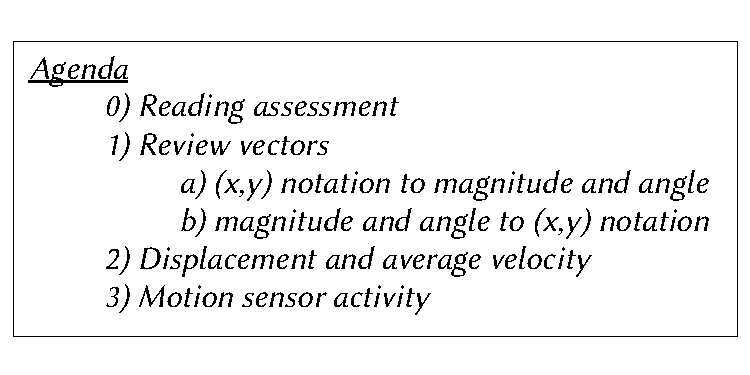
\includegraphics[width=0.45\textwidth]{ExampleAgenda.pdf}
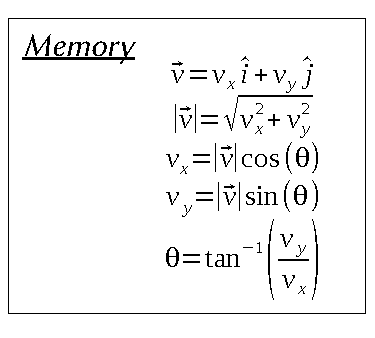
\includegraphics[width=0.22\textwidth]{ExampleMemory.pdf}
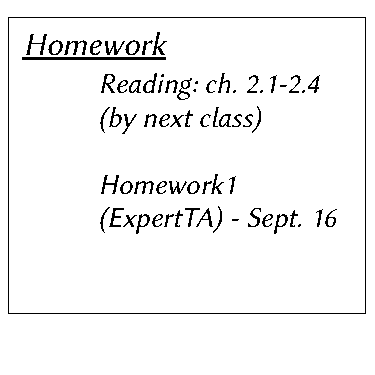
\includegraphics[width=0.22\textwidth]{ExampleHomework.pdf}
\caption{\label{fig:courses:intro:exampleAgenda} (Left) The class agenda presented on the white board is always concise and based on student progress.  It is presented to the students before each class period.  (Middle) The memory bank is a list of equations on the whiteboard used during class, and is a practice that I began using in 2017.  (Right) The homework box on the whiteboard now includes specific reading assignments, in addition to placing them on the syllabus.  This practice follows the suggestion of a student from a 2018 section of algebra-based physics (135A).}
\end{figure}

To structure class, I prepare my whiteboard in the pattern shown in Fig. \ref{fig:courses:intro:exampleAgenda}.  After explaining the agenda and homework, class begins with a reading assessment or the bonus article disussion mentioned above.  This is followed by warm-up examples from the memory bank (see Fig. \ref{fig:courses:intro:exampleAgenda}).  Next, I introduce new concepts on the projector screen, followed by several examples in traditional form on the whiteboard.  Third, I engage the students with a PI module pertaining to the concept just presented in traditional form.  PI modules begin with an exercise on the screen, with A-D multiple choice.  Our classrooms have a system that records student answers anonymously, and the students first answer individually.  I display the answer distribution (see Fig. \ref{fig:exampleData} below), and if fewer than 70\% of the class answers correctly I initiate \textbf{table discussions} (see Sec. \ref{sec:moduleType}).  \\ \hspace{0.1cm}

PER shows that students learn efficiently from peers explaining their reasoning.  Table discussions encourage this type of learning and  give me the chance to find the struggling students. Spending time with struggling students helps me build a relationship of trust, and relaxes their anxieties.  After short table discussions, students submit their answers again.  We observe the answer distribution shift toward the correct one (see Fig. \ref{fig:exampleData}).  Further, if 70\% of students answer correctly, we move forward.  Thus, we accelerate the pace if the students understand.  This creates the possibility of a few students being left behind, so I have added the concept of WAT\footnote{e.g. ``What?'' A meme indicating confusion.}.  WAT corresponds to answer E.  If I observe a WAT, I provide additional example work.  \textit{This strategy ensures inclusivity}, in that we strive to leave no one behind in class.  \\ \hspace{0.1cm}

The second-half of the lecture/laboratory format moves on to the lab activity or PhET module.  An example of the interplay between  labs and PhET occurs in PHYS135B and PHYS180 (electromagnetism).  As part of these courses, we build DC electric circuits.  If the circuit is constructable in our lab, we perform a traditional experiment to measure voltages and electric current to verify Ohm's Law\footnote{Ohm's law states that the current observed is proportional to the voltage in the circuit.}.  If the circuit cannot be easily built in our lab, we simulate it virtually with PhET software.  Whenever possible, we first simulate the circuit in PhET, and then construct it to compare simulation and experiment.  The PI modules, PhET modules, and traditional lecture content complete my strategy for improving the students' analysis skill, and go towards \textbf{Departmental goals 1, 4, and 6}.  \textit{The student evaluation data in Sec. \ref{sec:oof} show great progress in the student evaluation questions pertaining to this learning focus.} \\ \hspace{0.1cm}

I employ several methods to reach my third introductory course learning focus, \textbf{applications to society}.  The obvious routes are the applications in the OpenStax texts \cite{openstax1} regarding kinesiology and medicine.  I develop special PI modules and example problems around topics such as motion/work/energy in the human body, nerve cells as DC circuit simulation, and lightning/weather.  Which modules I deploy depends on the semester.  After reflecting on recent semesters, I have noticed that learning what interests the students and including content specifically pertaining to their majors is highly beneficial to keep them engaged.  Dropping the JITT module also frees more class-preparation time to add material I know particular students will enjoy\footnote{See supplemental material for an example of such a unit.}. \\ \hspace{0.1cm}

Two final methods for my third learning focus are the article discussions and term-papers.  An example of the former occured during the past year when an environmental science major in PHYS135A/B regularly tied physics to climate change by presenting geophysics articles.  These presentations empower the students to choose topics they know to have an impact on our community.  Occasionally I suggest high-impact articles and offer extra credit, and these prompts encourage shy students to prepare one.  I also offer extra-credit for term-papers asking students to explain the physics of a recent or past historical discovery.  Some brilliant examples have emerged, including the history of the first measurement of the distance to the Sun\footnote{Included in the supplemental material.}.  The story of these first measurements is connected to the first explorations of Antarctica, and I have included this astronomy/Antarctica connection in INTD255.  The students use course concepts to understand scientific breakthroughs, and it provides them a venue to practice technical writing (\textbf{Departmental goal 7}).  \\ \hspace{0.1cm}

\textbf{\textit{Calculus-based physics (150/180)}}. Calculus-based physics, PHYS150/PHYS180, is a two-semester lecture/laboratory formatted sequence that covers calculus-based kinematics, mechanics, work/energy, and electromagnetism\footnote{See supplemental material for example syllabi.}.  The format of these courses is similar to algebra-based physics, mixing PER and traditional content \textbf{departmental goals 1, 4, and 6}.  I employ PI modules \cite{mazur2013peer} and PhET modules \cite{phet}.  In addition, these courses require tools from calculus\footnote{MATH141/142 may be taken concurrently.}.  Students new to calculus benefit from PhET tools, which help to visualize calculus concepts\footnote{This is especially important in PHYS180 when PhET helps to visualize electromagnetic fields, a concept from MATH241.}.  My total teaching credits and number of students for this course is listed in Tab. \ref{tab:courses:teaching}. \\ \hspace{0.1cm}

My PHYS150/180 classes are taught in the same fashion as PHYS135A/B, but include the calculus intrinsic to introductory physics.  Calculus and Newton's Laws were developed concurrently, often by the same people, making them interconnected.  I occasionally pose a calculus problem during the warm-up or reading assessment phase of class, because I need to familiarize the students with a technique that helps solve physics problems in the current chapter.  Occasionally the physics requires concepts that the students will first encounter in Calculus III, or MATH241 (which covers electromagnetic fields).  I gauge the comfort level of the students, and typically restrict my calculus content to traditional examples or an occasional PI module.  \textit{As a rule, we do not place calculus concepts on exams that the students have not encountered in pre-requisite or concurrent courses}.  \\ \hspace{0.1cm}

In Sec. \ref{sec:oof}, I reflect on the student evaluation data in the same fashion as with the algebra-based courses.  Similar to the conclusions for PHYS135A/B, the data in Sec. \ref{sec:oof} show that calculus-based students are reporting an increase in their curiosity for physics over time, and \textit{great progress in measures touching upon their problem solving skills.}  I received almost perfect scores for data collected from my most recent PHYS180 course.  Although the reduced class size helped, I have reflected on the fact that the students place a high value on \textit{building a relationship of trust with them} in order to satisfy their curiosity and increase their analysis abilities.

\subsubsection{Descriptions of each Module Type}
\label{sec:moduleType}

The PI and PhET modules are outlined below for more detail and clarity, since it is likely that they are only familiar to physics instructors. \\ \hspace{0.1cm}

\underline{PI Modules} - An active learning strategy involving group problem solving and discussion \cite{mazur2013peer} \cite{AAPTPI} \cite{PhysPort}.  Figure \ref{fig:exampleData} contains data relevant to the following example.
\begin{itemize}
\item PI-based modules contain multiple-choice questions about a physical system.  Suppose we ask the students the following question: \\ \vspace{0.5cm} \textbf{If the slope on a graph of $x(t)$ vs. $t$ is positive before $t_0$, zero at $t_0$, and negative after $t_0$, \\ \vspace{0.5cm} A) the acceleration of the object was negative before and after $t_0$.  \\ B) the acceleration of the object was positive before $t_0$, then negative. \\ C) the acceleration of the object was positive before and after $t_0$. \\ D) the object had no acceleration.}
\item Each student responds \textit{anonymously} with a device, and their answers appear on-screen (see Fig. \ref{fig:exampleData}).
\begin{figure}
\centering
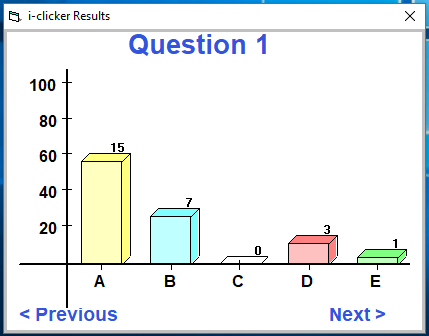
\includegraphics[width=0.45\textwidth,trim=0.25cm 1cm 0.15cm 2cm,clip=true]{FirstData.PNG}
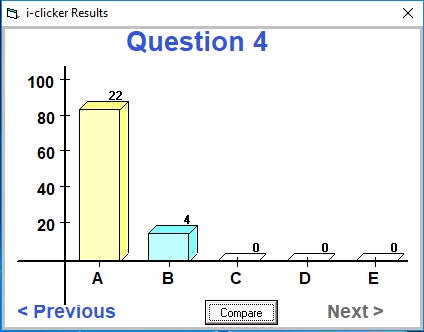
\includegraphics[width=0.45\textwidth,trim=0.25cm 1cm 0.15cm 2cm,clip=true]{SecondData.PNG}
\caption{\label{fig:exampleData} (Left) An answer distribution of my 25-student PHYS135A class (A was correct).  This distribution triggered a table discussion.  One student pressed E (indicating confusion) and I took appropriate action.  (Right) After table discussions, the students responded and the fraction of correct answers was 22/25 = 0.88.}
\end{figure}
\item Students know to press E if they are confused.  As described in the text, this maintains inclusivity in class.
\item One of two actions is taken next:
\begin{enumerate}
\item If the fraction of correct answers is $>0.7$, we proceed to the next exercise or new material\footnote{The number 0.7 was the recommended fraction at the American Association of Physics Teachers (AAPT) conference I attended in 2017.}.
\item If the fraction is $<0.7$, the professor initiates \textbf{table discussion}.
\end{enumerate}
\item \textbf{Table discussions} take place between students at the same table.  During this time the professor circulates, searching for and helping the struggling students.  After 3-5 minutes, the discussion ends.
\item A second poll of the class is taken after table discussions.  The \textit{shift} in the distribution towards the correct answer indicates improved understanding.  The professor takes appropriate action if there is not a shift.  If there are WATs (answer E), the material is re-addressed.
\item The procedure is repeated for several exercises, and table discussions take place when necessary.  After several exercises, the class proceeds to new material. See Fig. \ref{fig:exampleData} for example PI data.
\end{itemize}

\underline{PhET Modules} - These are interactive simulation tools published by The University of Colorado, Boulder \cite{phet}.  They are based on proven PER and written such that any student can operate them.
\begin{itemize}
\item The OpenStax textbooks for our courses have built-in links to PhET tools, allowing students to illustrate concepts by visually.
\item Several HTML5-based examples are here:
\begin{enumerate}
\item Electric charge and electric field: \url{https://phet.colorado.edu/en/simulation/charges-and-fields}
\item DC circuits: \url{https://phet.colorado.edu/en/simulation/circuit-construction-kit-dc}
\end{enumerate}
\item PhET simulations are incorporated into active learning in the classroom in four situations:
\begin{enumerate}
\item When a PhET tool re-creates a laboratory measurement, it is useful and informative to first simulate the expected results and then compare to the real ones.
\item PhET tools are used when an experiment cannot be constructed in the lab, such as altering gravity or changing the friction between surfaces.  Students benefit by being able to fine-tune a system in order to understand it.
\item PhET tools are used to \textit{visualize} systems which are invisible.  Examples are magnetic, electric, and gravitational fields, which are real but not always visible.
\item In special units, such as studying the behavior of electrical signals in the human body, there are useful PhET tools from biology, chemistry, medicine, and earth science that help me engage the curiosity of students.
\end{enumerate}
\end{itemize}

\end{document}

